\section{Player Types}
\label{chap:player_types}

Understanding player types and motivations are essential for designing games. This is because changes in game business practices have elevated the need for distinguishing player types and player styles, similar to how segmentation is used in marketing. Players can have very different interests in playing, which are important to consider when designing games. This chapter takes a look at \citeauthor{hamari_player_2014}'s player types (\citeyear{hamari_player_2014}). The article presents different approaches and understandings of player topologies found in previous literature. 

The use of segmentation has always been a central part of marketing practices. This practice implies that products are designed with specific end-users in mind as opposed to mass-marketing. The goal of segmentation is to identify homogeneous customers, to offer products that better match their needs. There are four categories of segmentation established in marketing theory; geographic, demographic, psychographic, and behavioral segmentation. \textit{Geographic} segmentation divides people into groups based on their geographical region. \textit{Demographic} segmentation divides people into groups based on descriptive features such as age, gender, occupation, and education. \textit{Psychographic} segmentation divides people based on personal traits, such as attitude, interests, lifestyle, and values. And, \textit{Behavioral} segmentation categorizes people into groups based on behavioral patterns observed in people.

Out of the four categories, geographic and demographic segmentation have not been of primary interest due to their irrelevance to game design. \citet{hamari_player_2014} explicitly states that their review attempts to conceptualize motivations, behavior, and traits that categorize within the psychographic and behavioral segments. The two segmentation categories are often challenging to distinguish, and \citet{hamari_player_2014} states that the literature interprets these differently. The game genres covered in \citet{hamari_player_2014} vary; however, Massive Multiplayer Online (MMO) games are more recurring than others.

\subsection{Bartle's Four Archetypes}
Though \citet{hamari_player_2014} review several papers on player topologies, many of them seem to stem from the core principles of Bartle’s four player types  (\citeyear{bartle_hearts_1996}). The player types, also known as Bartle’s taxonomy, are the result of observations Bartle made in player behavior in Multi-User Dungeons (MUDs). Through his observations, he created a two-dimensional model where each quadrant represents a player type, see Figure \ref{fig:bartle_playertypes}. The model’s two dimensions to playing are action vs. interaction, and player-orientation vs. world-orientation. Based on players’ position on the axes, one can distinguish players into the four player types; \textit{Achievers}, \textit{Explorers}, \textit{Killers}, and \textit{Socializers}. An Achiever is a player that prefers world-oriented actions to achieve measurable rewards like points. An Explorer is a player that prefers interaction in the game world, like discovering new areas. A Killer is a player that prefers action towards other players and thrives on competition. And a Socializer is a player that prefers interaction with other players over the game itself.

\begin{figure}[H]
    \centering
    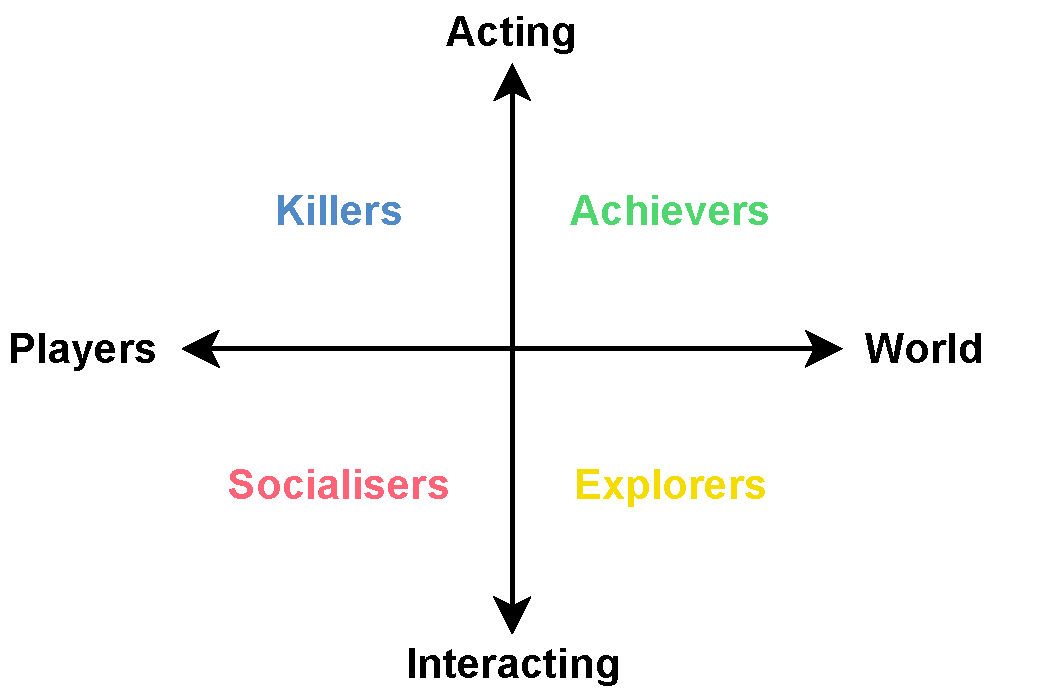
\includegraphics[width=0.7\textwidth]{Images/Theory/BartlesPlayerTypes.pdf}
    \caption{Bartle’s player types model \citep{bartle_hearts_1996}.}
    \label{fig:bartle_playertypes}
    \vspace*{-0.7\baselineskip}
\end{figure}

Although Bartle’s model on player types is insightful, it has received criticism for being too generalizing. Besides, it does not consider that players can have multiple motivations or that their motivations for playing may change over time, making it difficult to pinpoint a player type. \citet{hamari_player_2014} emphasizes that the criticism stems from how the topologies have been used and suggests that the dimensions can be used as scales rather than nominal categories.

\citeauthor{hamari_player_2014} also review the work of \citet{yee_motivations_2007}, where he observed player motivations in MMORPGs. \citet{yee_motivations_2007} builds on \citet{bartle_hearts_1996}, however, Yee suggests that there are only three main motivational factors of motivation, with additional sub-factors. The main factors are Achievement, Social, and Immersion. Yee’s underlying facets of Achievement and Social have a resemblance to Bartle’s heuristics found in Achievers, Explorers, and Socializers; however, they are not perfectly comparable. Moreover, \citeauthor{bartle_hearts_1996} did not consider Immersion explicitly, while \citeauthor{yee_motivations_2007} found that immersion was a major motivational factor for players.

\subsection{Hamari and Tuunanen’s Proposed Dimensions}
The review on player topologies is extensive; however, it is surprisingly uniform. Hamari and Tuunanen suggest that the results can be summarized as seven dimensions, based on recurring ideas from the reviewed papers.

\paragraph*{Achievement}
\textit{\footnotesize Related keywords: Achiever, Single-oriented player, Guardian/Achiever, Aggressive gamer, Achievement, Progress \& provocation, Power \& domination, Runner, Hard fun, Casual, Avatar level, (Semi-)professional.}

The achievement dimension focuses on single world-oriented players that thrive on rewards, progress, provocation, and power. 
    
\paragraph*{Exploration}
\textit{\footnotesize Related keywords: Explorer, Solver, Rational/Explorer, Aggressive gamer, Social gamer, Immersion, Exploration \& fantasy, Story \& escapism, Curiosity.}

The Exploration dimension is about exploring the game world. The players are driven by curiosity, fantasy, and storyline to escape the real world.
    
\paragraph*{Sociability}
\textit{\footnotesize Related keywords: Socialiser, Social mentalities, Community-oriented player, Idealist/Socialiser, Social, Helping \& support, the people factor, Friends \& collaboration, (Semi-)professional, Amateur.}

The Sociability dimension is about community-oriented players who enjoy and are motivated by other players’ support and presence. 
    
\paragraph*{Domination}
\textit{\footnotesize Related keywords: Killer, Artisan/Killer, Aggressive gamer, Off-real world-oriented player, Progress \& provocation, Power \& domination, Casual.}

The domination dimension is about the player’s need for aggressive gameplay. This could be players trying to accumulate as much gear as possible or damage others, leading to the underlying desire of feeling powerful.

\paragraph*{Immersion}
\textit{\footnotesize Related keywords: Immersion, Committed mentalities, Exploration \& fantasy, Story \& escapism, Off-real world-oriented player, Altered states, Hardcore.}

The Immersion dimension is about the degree to which players are committed and immersed in the game. Players may be driven by exploration, story, and fantasy. 
    
\paragraph*{Gaming intensity and skill}
\textit{\footnotesize Related keywords: Hardcore, Committed mentalities, Aggressive gamer, Veteran, Casual, Casual mentalities, Inactive gamer, Pacifist, Avatar level, Amateur.}

The Gaming Intensity and skill dimension are about the player’s commitment, experience, and attitude towards the game. Players are often said to be casual or hardcore players. Hardcore players are usually experienced and highly skilled, whereas casual players might be less experienced and less committed.  Players are placed by their willingness to participate, make an effort, and play.
    
\paragraph*{In-game demographics}
\textit{\footnotesize Related keywords: Avatar class and profession, non-clan member, Amateur, Professional, Group centrality, Size of the guild, Type of server, Faction.}

The In-game demographics dimension is about the player’s progress vs. their role. Examples of this can be different avatar classes, in-game professions, and positions in the hierarchy. For instance, players can pursue to level up their avatar from warrior to king as they progress in the game.

Though the papers are not directly comparable, because of their different scope, Hamari and Tuunanen go on to suggest that these seven recurring dimensions can instead be considered as five key dimensions and two supporting dimensions of player motivations. Achievement, Sociability, Exploration, Domination, and Immersion are the five key dimensions, and Game intensity and In-game demographics are the supporting dimensions. The reasoning behind this seems to be about the motivation of play. Achievement and Sociability seem to be the most recurring concepts in the literature; Immersion and Domination appear in some papers, whereas In-game demographics were only found in a few papers.

\subsection{Player Types and Reward Characteristics}
In the light of Hamari and Tuunanen’s player types, it is logical to see this in context with \citet{wang_game_2011} work on reward systems, previously discussed in Chapter \ref{chap:reward_systems}. \citet{wang_game_2011} review also presents four reward characteristics that can be used to analyze the influence of reward systems on different kinds of players.

The first one, social value, can be used for comparison of players or social interaction. This type of reward characteristic is particularly attractive for Socializers and Achievers. Rewards in games make it easier for players to compare themselves against others. An example is a high score list. The player can compare their points to others to see how they rank. Another good example is how hard-to-get items often draw attention. 

The next characteristic looks at "how rewards affect gameplay”. For this particular characteristic, it is interesting to see how rewards can help the player advance in the game, motivate them to produce new content, and participate in the game. Using the player types from Bartle’s taxonomy, \citet{wang_game_2011} summarizes the effect reward has on different player types as:

\begin{itemize}
    \item \textbf{Achievers and Killer:} Most interested in accumulating rewards that are evidence of their advanced skills and do not care about the visual aspect.
    \item \textbf{Socializers:} Greater interest in rewards that can draw attention to them, e.g., hard to get items.
    \item \textbf{Explorers:} Like Achievers and Killers, the motivation behind is gaining sufficient strength to explore game world details.
\end{itemize}

The third attribute is "suitability for collection and review” \citep{wang_game_2011}. The logic behind this is that building a sense of accomplishment improves the ability to preserve game memories. Collecting rewards is also a tool for players to recognize other players with similar interests. An important design consideration for this attribute is to showcase the rewards, so they are easy to present and review in the game. For instance, medals or badges that indicate game status or ranking can be showcased on the player’s profile. The rewards could then strengthen the sense of collection and produce a feeling of completion and perfection among the players.
The last characteristic is "the time required to earn and/or receive a reward" \citep{wang_game_2011}. In contrast to real-world rewards, e.g., job promotion, a game reward can be instantaneous or rewarded after a couple of hours of gaming. A player may, for example, get a new level as a reward after a couple of hours of play. The time and intensity required to earn a reward are crucial aspects of game design that must be carefully planned to create a positive player experience.

Though most of the player topologies have been built on observations of MUDs, MMORPGs, and other online games, the topologies seem to be relevant for various game types. The results can, for instance, be applied in the context of gamification, where game mechanics related to sociability and achievements are frequently used. Some of these mechanics can be social rewards such as likes and comments or achieving good results, and breaking records for other players to see.

\subsection{Summary}
This chapter has introduced different interpretations of player types. We looked at the recurring ideas present in literature and have concretized them into seven primary dimensions. Depending on the game concept and genre, game designers may use Hamari and Tuunanen’s dimensions to create organic game environments that offer rewarding gameplay for different player types. The dimensions and understandings from this chapter will be useful later for developing new game concepts and for the design, development, and analysis of the final game.